\chapter{Конструкторская часть}

\section{Разработка стандартного алгоритма умножения матриц}
На рисунке \ref{img:simple} приведена схема стандартного алгоритма умножения матриц.
\begin{figure}[h]
	\centering
	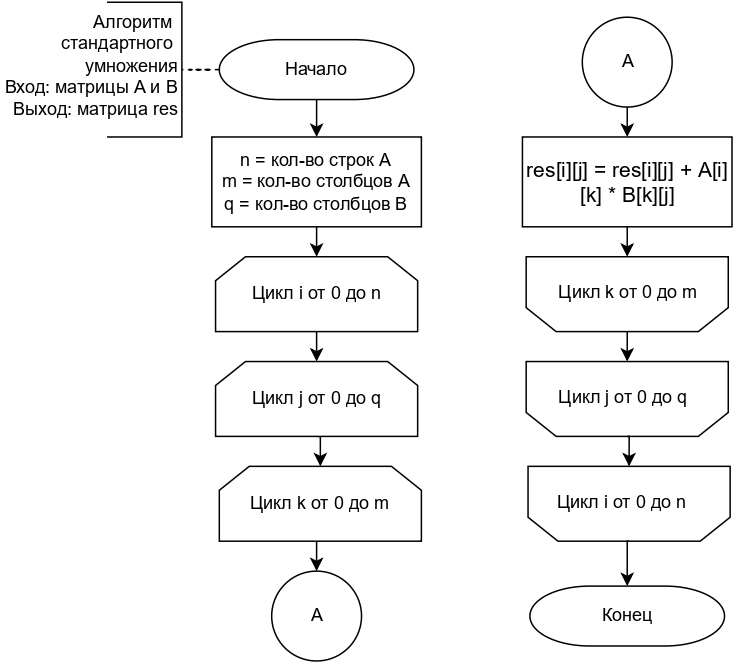
\includegraphics[width=140mm]{images/simple}
	\caption{Схема стандартного алгоритма умножения матриц}
	\label{img:simple}
\end{figure}

\section{Разработка алгоритма Винограда умножения матриц}
На рисунке \ref{img:grape} приведена схема алгоритма Винограда умножения матриц.
\begin{figure}[h]
	\centering
	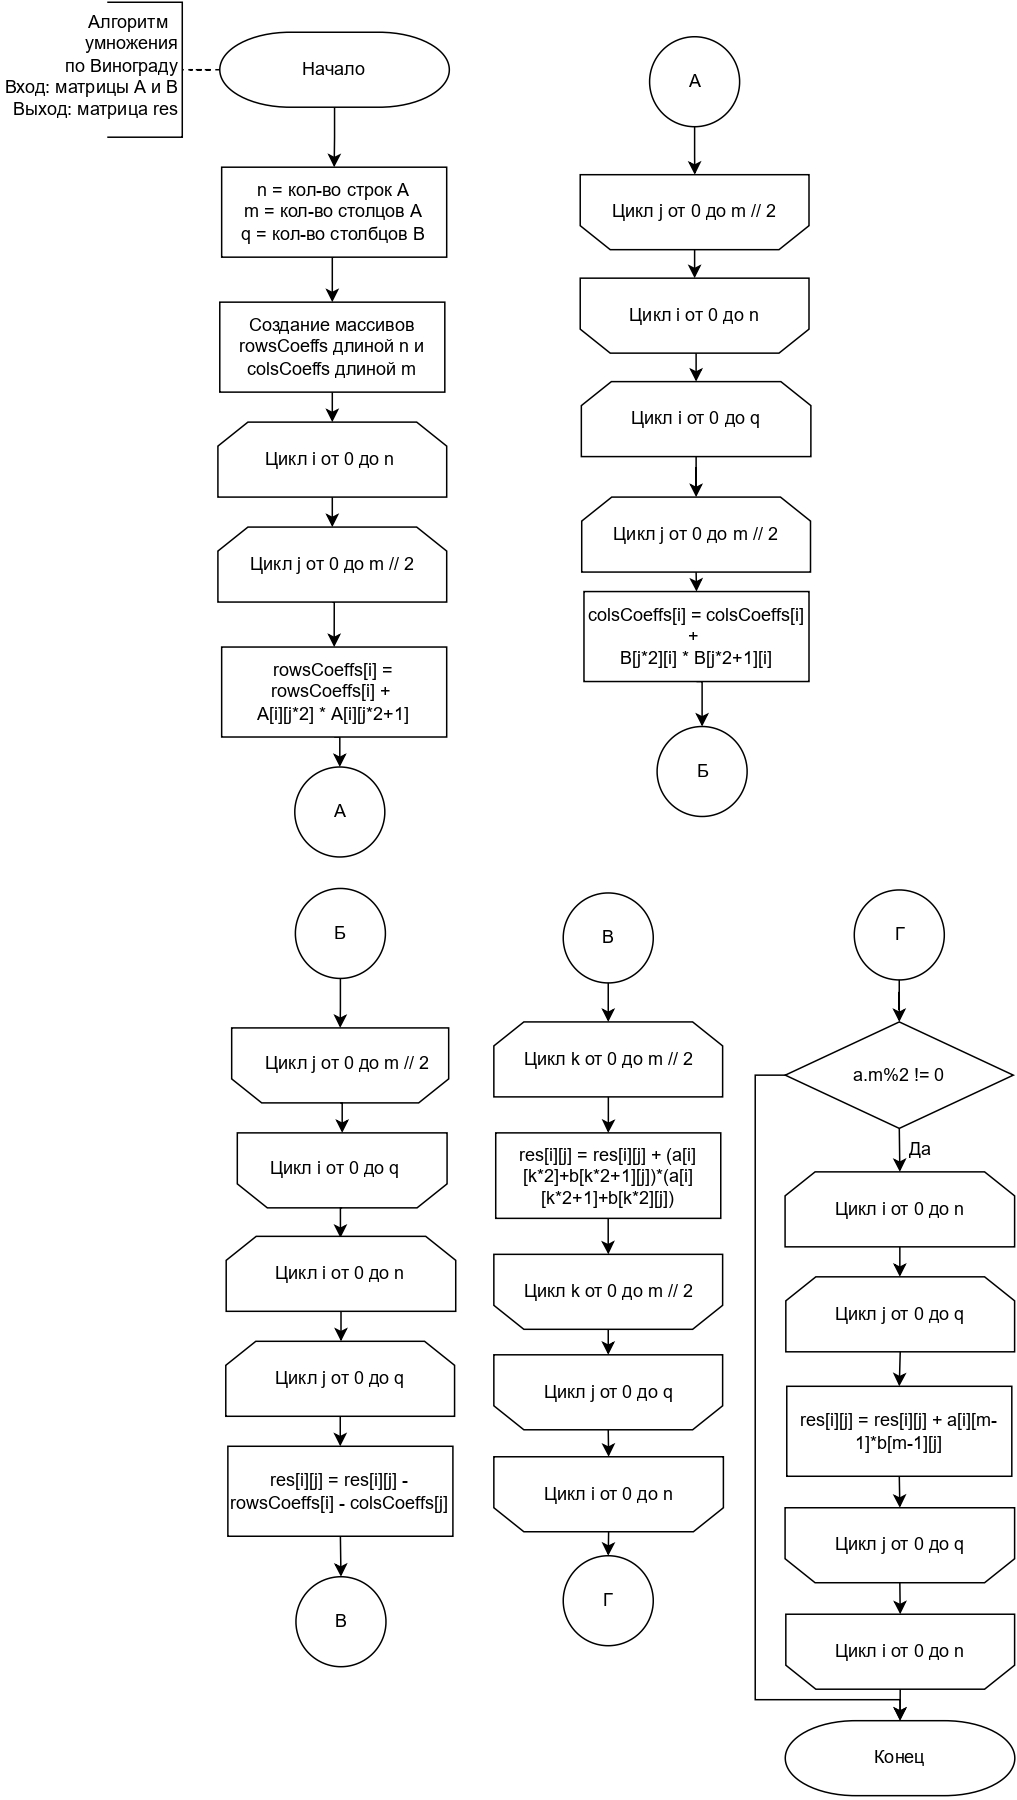
\includegraphics[width=130mm]{images/grape}
	\caption{Схема алгоритма Винограда умножения матриц}
	\label{img:grape}
\end{figure}
\clearpage
\section{Разработка оптимизированного алгоритма Винограда умножения матриц}

На рисунке \ref{img:grapePro} приведена схема оптимизированного алгоритма Винограда умножения матриц.
\begin{figure}[h]
	\centering
	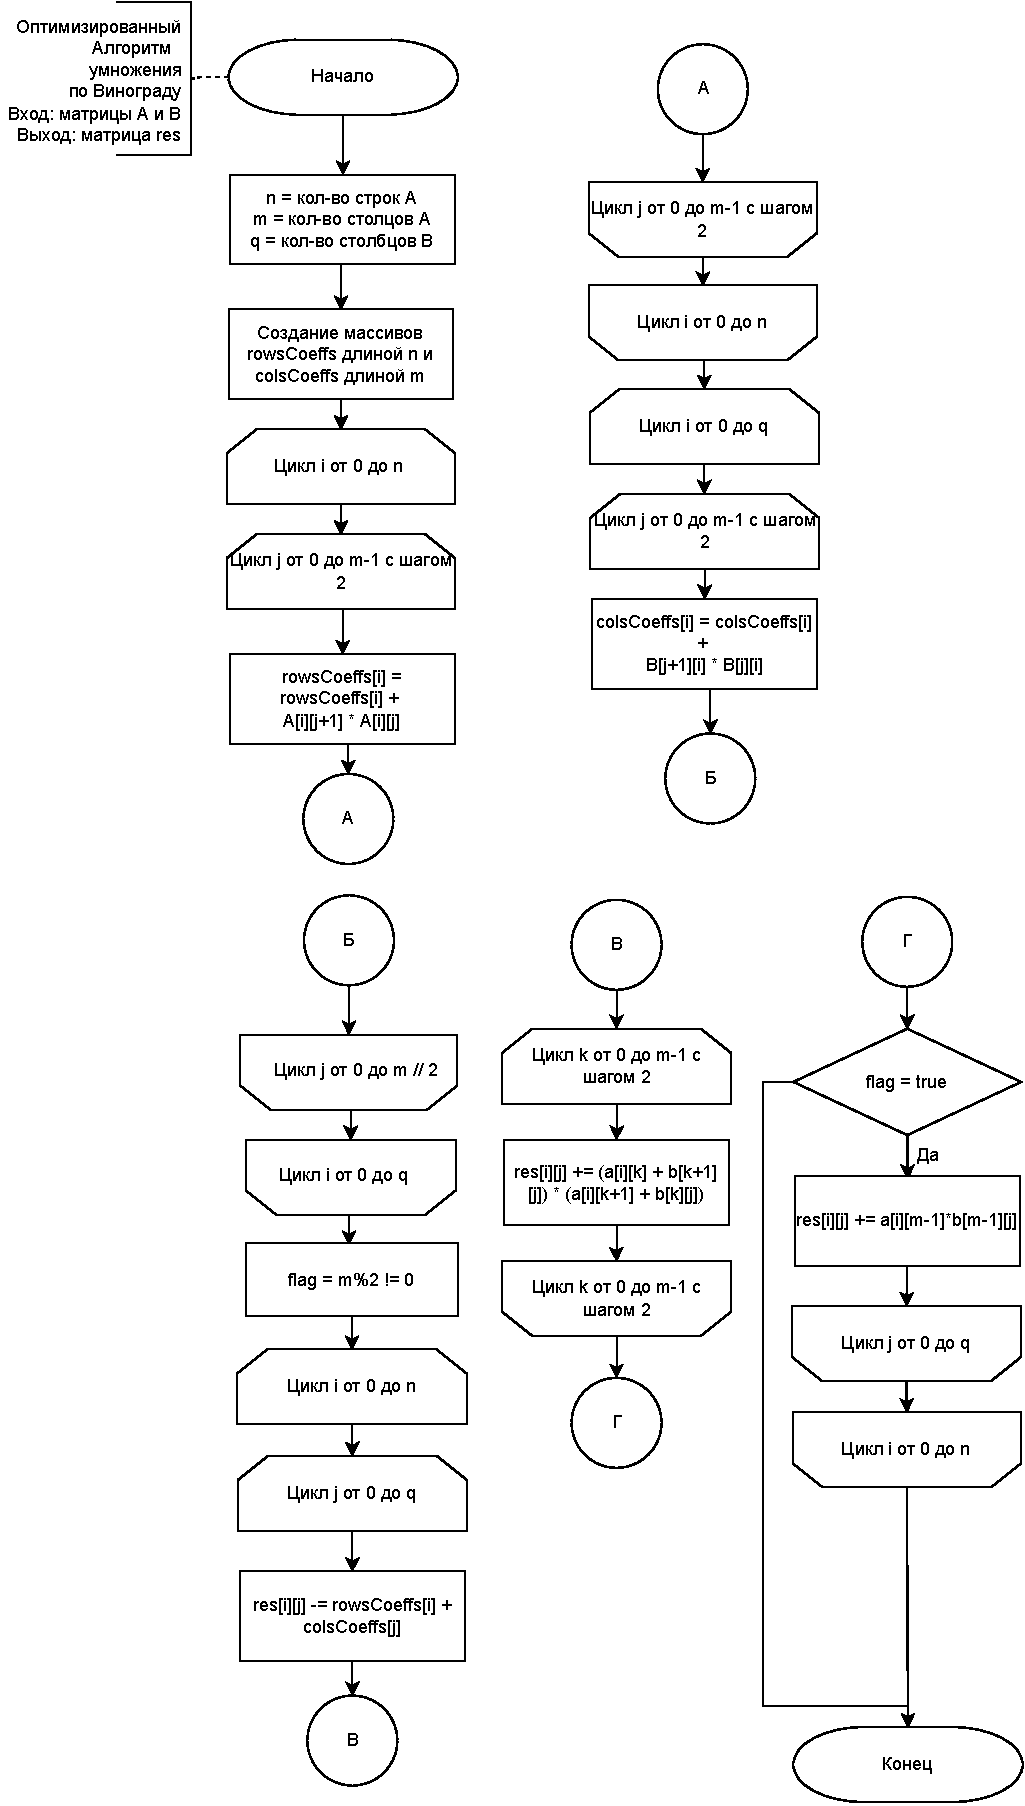
\includegraphics[width=100mm]{images/grapePro}
	\caption{Схема оптимизированного алгоритма Винограда умножения матриц}
	\label{img:grapePro}
\end{figure}

\clearpage
\section{Модель вычислений}

Для последующего вычисления трудоемкости необходимо ввести модель вычислений.

Операции из списка (\ref{for:opers}) имеют трудоемкость 1.

\begin{equation}
	\label{for:opers}
	=, +=, -=, +, -, ==, !=, <, >, <=, >=, [], ++, {-}-
\end{equation}

Операции из списка (\ref{for:opers2}) имеют трудоемкость 2.
\begin{equation}
	\label{for:opers2}
	*, /, \%
\end{equation}

Трудоемкость оператора выбора \code{if условие then A else B} рассчитывается как:
\begin{equation}
	\label{for:if}
	f_{if} = f_{\text{условия}} +
	\begin{cases}
		f_A, & \text{если условие выполняется,}\\
		f_B, & \text{иначе.}
	\end{cases}
\end{equation}

Трудоемкость цикла рассчитывается как:
\begin{equation}
	\label{for:for}
	f_{for} = f_{\text{инициализации}} + f_{\text{сравнения}} + N(f_{\text{тела}} + f_{\text{инкремента}} + f_{\text{сравнения}})
\end{equation}

Трудоемкость вызова функции равна 0.


\section{Трудоемкость алгоритмов}

Во всех алгоритмах создается дополнительная матрица, куда записывается результат. Трудоемкость инициализации не была учтена, так как это действие не является трудоемким.

\subsection{Стандартный алгоритм умножения матриц}

Трудоёмкость стандартного алгоритма умножения матриц состоит из следующих составляющих.

Трудоёмкость внешнего цикла по $i \in [0..M-1]$: $f = 2 + M \cdot (2 + f_{body})$.

Трудоёмкость цикла по $j \in [0..N-1]$: $f = 2 + N \cdot (2 + f_{body})$.

Трудоёмкость цикла по $k \in [0..K-1]$: $f = 2 + 11K$.

Учитывая, что трудоёмкость стандартного алгоритма равна трудоёмкости внешнего цикла, можно вычислить ее, подставив циклы тела:
\begin{equation}
	\label{for:standard}
	f_{standard} = 2 + M \cdot (4 + N \cdot (4 + 11K)) \approx 11MNK
\end{equation}

\subsection{Алгоритм Винограда умножения матриц}

Трудоёмкость алгоритма Винограда состоит из следующих составляющих.

Трудоёмкость создания и инициализации массивов MH и MV:
\begin{equation}
	\label{for:init}
	f_{init} = M + N
\end{equation}

Трудоёмкость заполнения массива MH:
\begin{equation}
	\label{for:MH}
	f_{MH} = 2 + K (2 + \frac{M}{2} \cdot 11)
\end{equation}

Трудоёмкость заполнения массива MV:
\begin{equation}
	\label{for:MV}
	f_{MV} = 2 + K (2 + \frac{N}{2} \cdot 11)
\end{equation}

Трудоёмкость цикла заполнения для чётных размеров:
\begin{equation}
	\label{for:cycle}
	f_{cycle} = 2 + M \cdot (4 + N \cdot (11 + \frac{K}{2} \cdot 23))
\end{equation}

Трудоёмкость цикла, для дополнения умножения суммой последних нечётных строки и столбца, если общий размер нечётный:
\begin{equation}
	\label{for:last}
	f_{last} = \begin{cases}
		2, & \text{размер чётный,}\\
		4 + M \cdot (4 + 14N), & \text{иначе.}
	\end{cases}
\end{equation}


Итого, для худшего случая (нечётный общий размер матриц) имеем:
\begin{equation}
	\label{for:bad}
	f =  f_{MH} + f_{MV} + f_{cycle} + f_{last}\approx 11,5 \cdot MNK
\end{equation}

Для лучшего случая (чётный общий размер матриц) имеем:
\begin{equation}
	\label{for:good}
	f =  f_{MH} + f_{MV} + f_{cycle} + f_{last} \approx 11,5 \cdot MNK
\end{equation}


\subsection{Оптимизированный алгоритм Винограда умножения матриц}

Оптимизированный алгоритм Винограда представляет собой обычный алгоритм Винограда, за исключением следующих оптимизаций:
\begin{itemize}
	\item вычисление происходит заранее;
	\item вместо деления на $2$ в условии циклов, используется увеличение счётчика циклов на $2$;
	\item последний цикл для нечётных элементов включён в основной цикл,
	используя дополнительные операции в случае нечётности N.
\end{itemize}


Трудоёмкость улучшенного алгоритма Винограда состоит из следующих составляющих.

Трудоёмкость создания и инициализации массивов MH и MV:
\begin{equation}
	\label{for:impr_init}
	f_{init} = M + N
\end{equation}

Трудоёмкость заполнения массива MH:
\begin{equation}
	\label{for:impr_MH}
	f_{MH} =  2 + K (2 + \frac{M}{2} \cdot 8)
\end{equation}

Трудоёмкость заполнения массива MV:
\begin{equation}
	\label{for:impr_MV}
	f_{MV} =  2 + K (2 + \frac{M}{2} \cdot 8)
\end{equation}

Трудоёмкость цикла заполнения для чётных размеров:
\begin{equation}
	\label{for:impr_cycle}
	f_{cycle} =2 + M \cdot (4 + N \cdot (11 + \frac{K}{2} \cdot 18))
\end{equation}

Трудоёмкость условия для дополнения умножения суммой последних нечётных строки и столбца, если общий размер нечётный:
\begin{equation}
	\label{for:impr_last}
	f_{last} = 
	\begin{cases}
		1, & \text{размер чётный,}\\
		4 + M \cdot (4 + 10N), & \text{иначе.}
	\end{cases}
\end{equation}

Итого, для худшего случая (нечётный общий размер матриц) имеем:
\begin{equation}
	\label{for:bad_impr}
	f = f_{MH} + f_{MV} + f_{cycle} + f_{last} \approx 9MNK
\end{equation}

Для лучшего случая (чётный общий размер матриц) имеем:
\begin{equation}
	\label{for:good_impr}
	f = f_{MH} + f_{MV} + f_{cycle} + f_{last} \approx 9MNK
\end{equation}

